% Begin the document and set up the style of the document
\documentclass{beamer}

% Install the required packages for the document 
\usepackage{envmath}
\usepackage{esvect}
\usepackage{graphicx}
\usepackage{gensymb}
\usepackage{tikz}
\usepackage[mathcal]{euscript}
\usepackage{geometry}
\usepackage{mathtools}
\usepackage{subdepth}
\usepackage{graphicx}
\usepackage{amsmath}
\usepackage{amscd}
\usepackage{amssymb}
\usepackage{amsfonts}
\usepackage{harpoon}
\usepackage[title]{appendix}
\usepackage{pgf}
\usepackage{tikz}
\usepackage{mathrsfs}
\usepackage{asyalign}
\usepackage{physics}
\usepackage{enumitem}
\usepackage{xhfill}
\usepackage{accents}
\usepackage{cite}
\usepackage{url}
\usepackage{csquotes}
\usepackage{wrapfig}
\usepackage{booktabs}
\usepackage{adjustbox}
\usepackage{caption}
\usepackage{minipage-marginpar}
\usepackage{calc}
\usepackage{lmodern}
\usepackage[tableposition=top]{caption}
\usepackage{ifthen}
\usepackage[utf8]{inputenc}
\usepackage{tikz-3dplot}
\usetikzlibrary{patterns}
\usetikzlibrary{arrows}

\renewcommand{\familydefault}{\sfdefault}

\newcommand{\indep}{\mathrel{\text{\scalebox{1.07}{$\perp\mkern-10mu\perp$}}}}
\newcommand{\p}{\mathbb{P}}
\newcommand{\e}{\mathbb{E}}
\newcommand{\ds}{\displaystyle}
\newcommand{\code}{\texttt}
\usetheme{Boadilla}

\title{Fractals}
\subtitle{Cantor Set}
\author{Keegan Gyoery}
\institute{UNSW}
\date{\today}

\begin{document}

\begin{frame}
	\titlepage
\end{frame}

\begin{frame}
	\frametitle{Fractals}
	\begin{itemize}
		\item<2->
		\begin{definition}
			A fractal is a curve or geometric figure that is infinitely self-similar.
		\end{definition}
		\item<3->
		\begin{definition}
			A fractal is a curve or geometric figure whose self-similarity dimension exceeds its topological dimension.
		\end{definition}
		\item<4->
		\begin{definition}
			A fractal is a curve or geometric figure that is bounded, continuous and nowhere differentiable in some region $\ds{R}$.
		\end{definition}
	\end{itemize}
\end{frame}

\begin{frame}
	\frametitle{Examples}
	\begin{minipage}[t]{0.48\linewidth}
        \begin{itemize}
            \item<2-> 
            \centering
            \begin{figure}
            	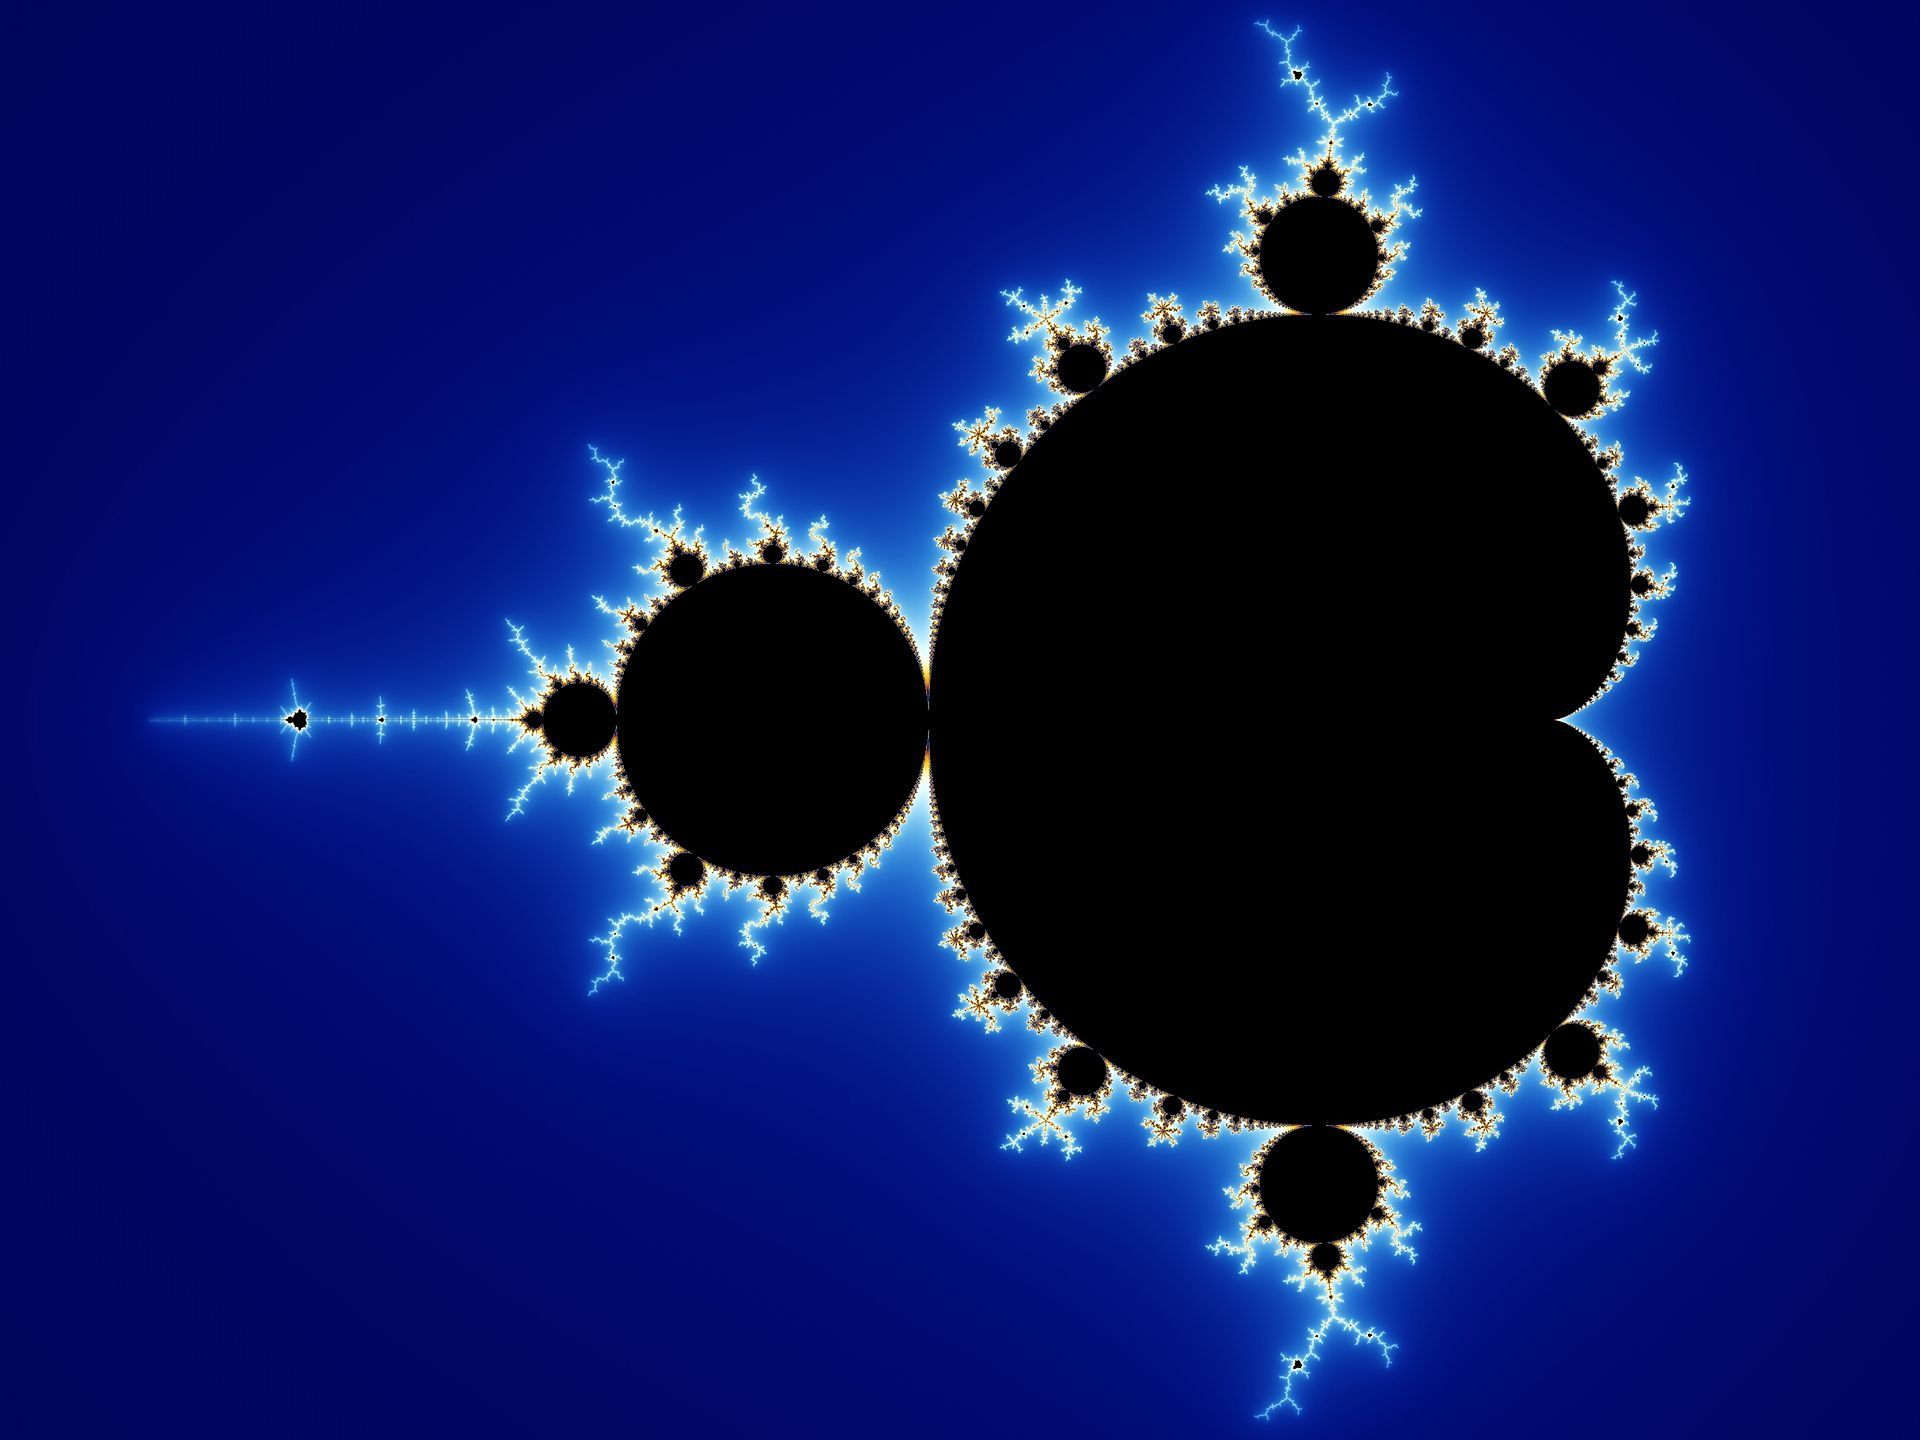
\includegraphics[width=5cm]{mandlebrot}
            	\caption{Mandlebrot Set}
            \end{figure}
        \end{itemize}
    \end{minipage}
    \hfill
    \begin{minipage}[t]{0.48\linewidth}%
        \begin{itemize}
            \item<3-> 
            \centering
            \begin{figure}
            	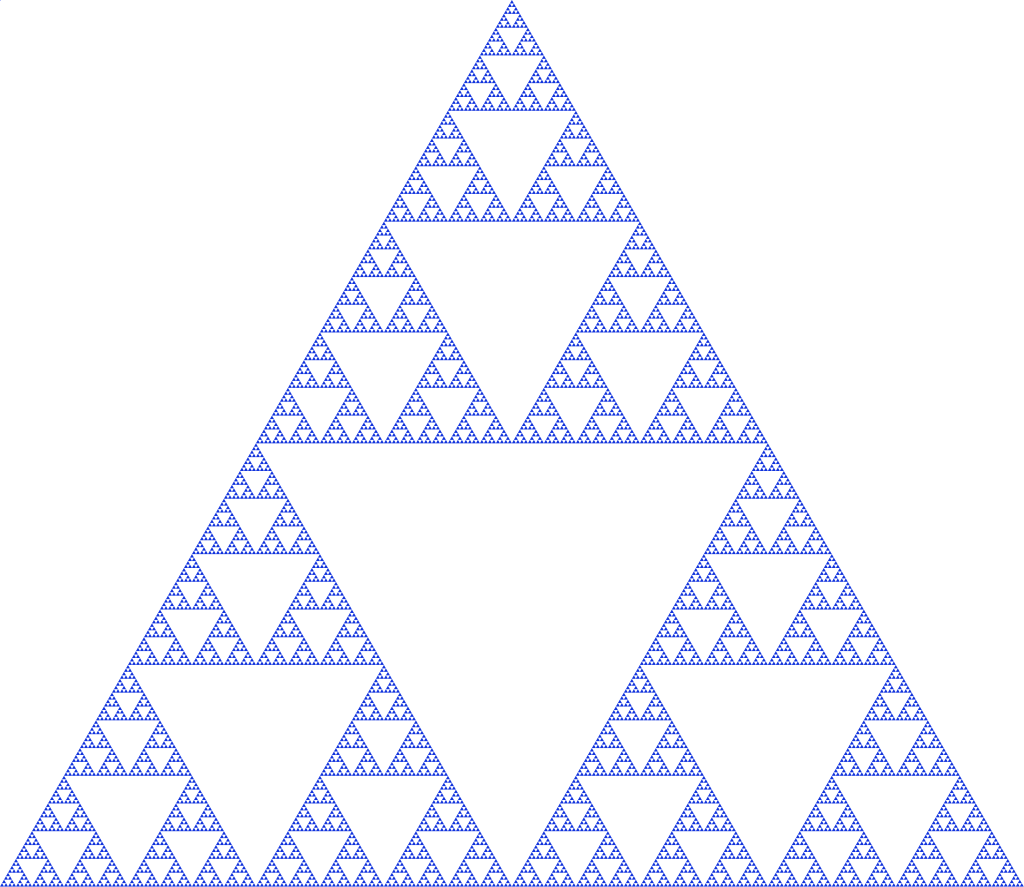
\includegraphics[width=5cm]{serpinski}
            	\caption{Serpinski Triangle}
            \end{figure}
        \end{itemize}
    \end{minipage}
\end{frame}

\begin{frame}
	\frametitle{Generation}
	\begin{itemize}
		\item<2->
		\begin{block}{Generation Steps}
			1. Start with a curve, or image.\\
			2. Apply a sequence of transformations that are repeatable to the curve, or image.\\
			3. Repeat ad infinitum.\\
		\end{block}
		\item<3->
		\begin{example}
			Cantor Set
		\end{example}
	\end{itemize}
\end{frame}

\begin{frame}
	\frametitle{Cantor Set}
	\begin{itemize}
		\item<2->
		\begin{theorem}
			The Cantor Set contains no interval of non-zero length, but is non-empty.
		\end{theorem}
		\item<3->
		\begin{proof}
			Consider the end points of the closed intervals at each step. These points remain, proving the Cantor Set is non-empty.\\
			Consider now the length of the open interval removed at step $\ds{n}$. The length of such an interval is $\ds{3^n}$. At step $\ds{n}$, $\ds{2^{n-1}}$ intervals are removed, and so the length of intervals removed is,
			$$\sum^{\infty}_{n=1}\frac{2^{n-1}}{3^n} = \frac{1}{3}\sum^{\infty}_{k=0}\frac{2^{k}}{3^k} = \frac{1}{3}\frac{1}{1-\frac{2}{3}} = 1$$
		\end{proof}
	\end{itemize}
\end{frame}

\begin{frame}
	\frametitle{Cantor Set cont.}
	\begin{itemize}
		\item<2->
		\begin{definition}
			The self-similarity dimension of a fractal is given by 
			$$\frac{\log N}{\log{\frac{1}{r}}}$$
			where $\ds{N}$ is the number of self-similar copies, and $\ds{r}$ is the scaling factor of the self-similar copies.
		\end{definition}
		\item<3->
		\begin{block}{Property}
			The topological dimension of the Cantor Set is 0, as it contains no intervals of non-zero length. The self-similarity dimension of the Cantor Set is $\ds{\frac{\log 2}{\log 3}}$. Thus, the Cantor Set is a fractal.
		\end{block}
	\end{itemize}
\end{frame}

\begin{frame}
	\frametitle{Consequences}
	\begin{itemize}
		\item<2->
		\begin{block}{}
		\setbeamertemplate{itemize items}[ball]
		\begin{itemize}
			\item - Countably infinite sets and their cardinality. 
			\item - Cardinality arithmetic.
			\item - Modelling of nature and natural phenomena.
			\item - Computer graphics and simulations.
		\end{itemize}
		\end{block}
	\end{itemize}
\end{frame}

\begin{frame}
	\frametitle{References}
	Cirstea, F. (2017). Fractals.\\
	Cirstea, F. (2017). Cantor Set.\\
\end{frame}


\end{document}